%% Tex spellcheck
% Maybe put this as Chapter 2

% Write in English.
\chapter{Chapter 3 : Simulations}

In this chapter, we will present the different simulations that were done to test the directivity and force of different coil shapes. There's is a wide variety diferrent software that can be used to simulate magnetic fields. I found Python scripting to be more versatile and easier to get the results I wanted.

The goal of these simulations is to determine if one shape is better than an other and if the magnetic field is strong enough to move a magnet. The simulations only take into account a fixed current of 1A and a number of turns in a determined area. We only really want the magnetic field in the X and Y direction as we will only move the magnet in a 2D space. But we should keep in mind that the Z direction might add some friction.

We'll do out calculations with a 6x6x6 cubic magnet with a magnetic field strength of 1.29T and a magnet weight of 1.6416 grams. We'll consider a friction coefficient of 0.2 for the magnet on the surface of the PCB.

In order to calculate the force of the magnetic field on the magnet, we'll need to compute the magnetic moment of a specific magnet, we need to know the volume of the magnet and the residual magnetism.

\begin{itemize}
	\item Residual magnetism: \( B_r = 1.29 \, \text{T} \)
	\item Side length of the cubic magnet: \( 6 \, \text{mm} = 0.006 \, \text{m} \)
\end{itemize}

The volume \( V \) of the cubic magnet is calculated as:
\[
	V = (\text{Side length})^3 = (0.006 \, \text{m})^3 = 2.16 \times 10^{-7} \, \text{m}^3
\]

The magnetic moment \( m \) is given by:
\[
	m = B_r \cdot V
\]
\[
	m = 1.29 \, \text{T} \times 2.16 \times 10^{-7} \, \text{m}^3
\]
\[
	m = 2.78 \times 10^{-7} \, \text{A} \cdot \text{m}^2
\]


\section{Linear coil}

\begin{figure}[H]
	\centering
	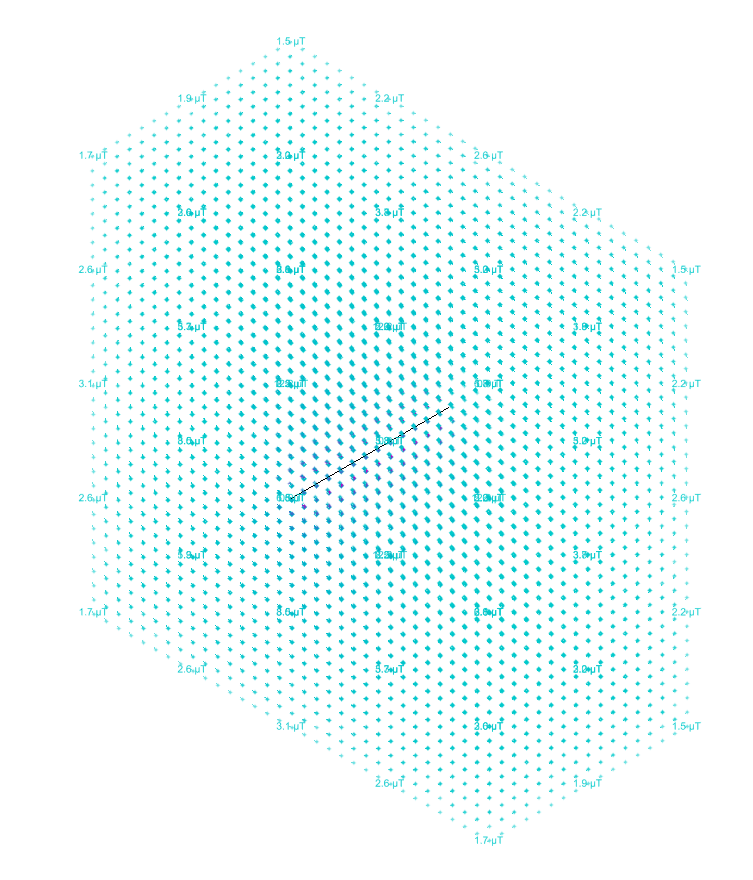
\includegraphics[width=0.8\linewidth]{simu_linear_coil.png}
	\caption[Simulation of a magnetic field in a simple wire]{Simulation of a simple wire in a 10mm x 10mm x 5mm zone, with a current of 1A}
	\label{fig:simu_simple_wire}
\end{figure}

As we can observe, the magnetic field is weak and gets weaker as we move away from the wire. We'll take a middle value of 8 uT at around 3mm from the wire.

Given data:
\begin{itemize}
	\item Magnetic flux density of the external field: \( B = 8 \, \mu\text{T} = 8 \times 10^{-6} \text{ T} \)
	\item Magnetic moment: \( m = 2.78 \times 10^{-7} \text{ A} \cdot \text{m}^2 \)
	\item Magnet weight: \( m_{\text{weight}} = 1.6416 \text{ g} = 0.0016416 \text{ kg} \)
	\item Coefficient of friction: \( \mu = 0.2 \)
	\item Acceleration due to gravity: \( g = 9.81 \text{ m/s}^2 \)
	\item Angle between magnetic moment and external field: \( \theta = 90^\circ \), so \( \sin(\theta) = 1 \)
\end{itemize}

Calculate the Magnetic Force

\[
	F_{\text{mag}} = m \cdot B \cdot \sin(\theta)
\]

\[
	F_{\text{mag}} = 2.78 \times 10^{-7} \, \text{A} \cdot \text{m}^2 \times 8 \times 10^{-6} \, \text{T}
\]

\[
	F_{\text{mag}} = 2.22 \times 10^{-12} \text{ N}
\]

Calculate the Friction Force

\[
	F_{\text{friction}} = \mu \cdot m_{\text{weight}} \cdot g
\]

\[
	F_{\text{friction}} = 0.2 \times 0.0016416 \text{ kg} \times 9.81 \text{ m/s}^2
\]

\[
	F_{\text{friction}} \approx 0.0032 \text{ N}
\]

Calculate the Total Force

\[
	F_{\text{total}} = F_{\text{mag}} - F_{\text{friction}}
\]

\[
	F_{\text{total}} = 2.22 \times 10^{-12} \text{ N} - 0.0032 \text{ N}
\]

\[
	F_{\text{total}} \approx -0.0032 \text{ N}
\]




\section{Circular or spiral coil}

\begin{figure}[H]
	\centering
	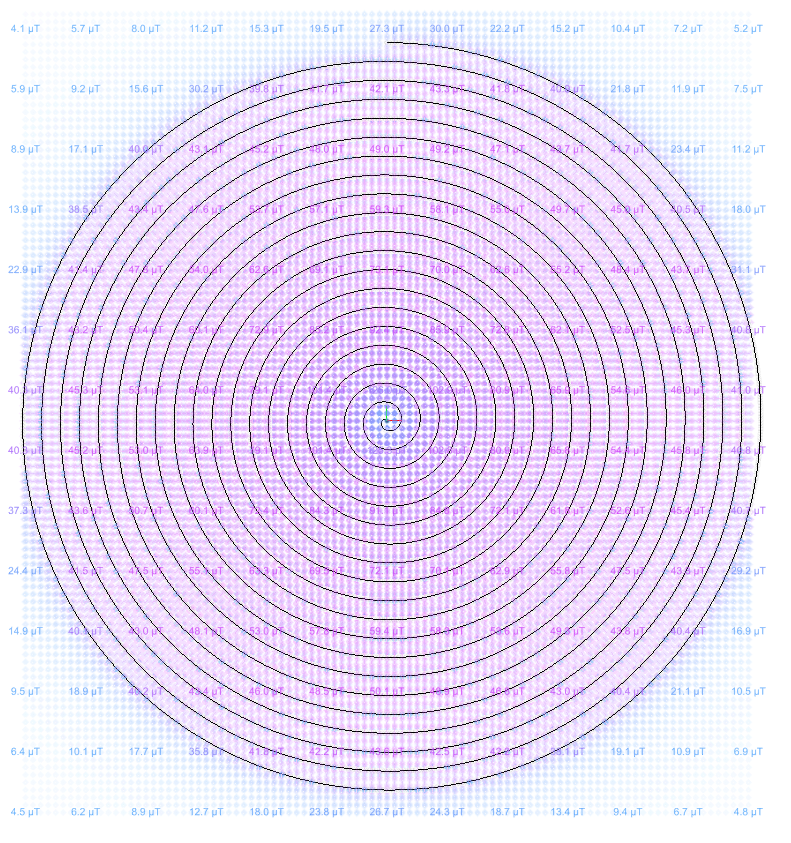
\includegraphics[width=0.8\linewidth]{simu_circular.png}
	\caption[Simulation the magnetic field in a spiral coil]{Simulation the magnetic field in a spiral coil with 20 turns for a total of 10mm diameter, with a current of 1A}
	\label{fig:simu_spiral}
\end{figure}

We'll take a middle value of 50 uT at around 3mm from the wire.

Given data:
\begin{itemize}
	\item Magnetic flux density of the external field: \( B = 50 \, \mu\text{T} = 50 \times 10^{-6} \text{ T} \)
	\item Magnetic moment: \( m = 2.78 \times 10^{-7} \text{ A} \cdot \text{m}^2 \)
	\item Magnet weight: \( m_{\text{weight}} = 1.6416 \text{ g} = 0.0016416 \text{ kg} \)
	\item Coefficient of friction: \( \mu = 0.2 \)
	\item Acceleration due to gravity: \( g = 9.81 \text{ m/s}^2 \)
	\item Angle between magnetic moment and external field: \( \theta = 90^\circ \), so \( \sin(\theta) = 1 \)
\end{itemize}

Calculate the Magnetic Force

\[
	F_{\text{mag}} = m \cdot B \cdot \sin(\theta)
\]

\[
	F_{\text{mag}} = 2.78 \times 10^{-7} \, \text{A} \cdot \text{m}^2 \times 50 \times 10^{-6} \, \text{T}
\]

\[
	F_{\text{mag}} = 1.39 \times 10^{-10} \text{ N}
\]

Calculate the Friction Force

\[
	F_{\text{friction}} = \mu \cdot m_{\text{weight}} \cdot g
\]

\[
	F_{\text{friction}} = 0.2 \times 0.0016416 \text{ kg} \times 9.81 \text{ m/s}^2
\]

\[
	F_{\text{friction}} \approx 0.0032 \text{ N}
\]

Calculate the Total Force

\[
	F_{\text{total}} = F_{\text{mag}} - F_{\text{friction}}
\]

\[
	F_{\text{total}} = 1.39 \times 10^{-10} \text{ N} - 0.0032 \text{ N}
\]

\[
	F_{\text{total}} \approx -0.0032 \text{ N}
\]

This means that the magnet is too heavy to move from the middle of the coil. We'll have to increase the magnetic field strength to move the magnet.


\section{rectangular coil}


\begin{figure}[H]
	\centering
	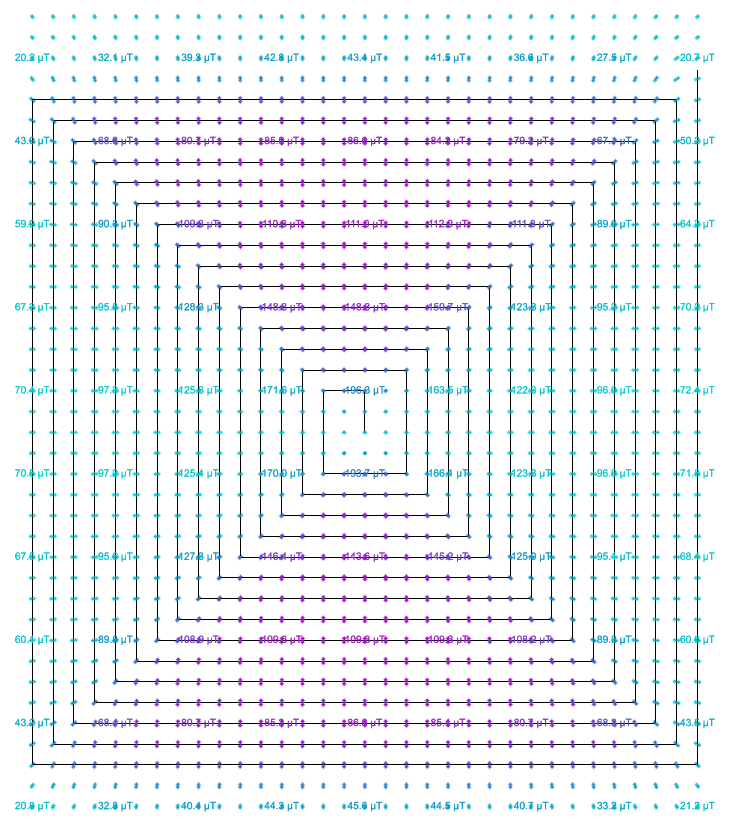
\includegraphics[width=0.8\linewidth]{simu_square_xy.png}
	\caption[Simulation of the magnetic field of a square coil]{Simulation of the magnetic field of a square coil with 15 turns for an area of 8mm x 8mm, with a current of 1A}
	\label{fig:simu_square}
\end{figure}

The forces applied on the magnet seem really weak, i might have issues with my calculations or the friction coefficient. The simulation are not showing what i can really see in real life.